% !TeX program = xelatex
% !TeX encoding = utf8
\documentclass[10pt,a4paper]{article}
\usepackage{fontspec}
\usepackage{polyglossia}
\setdefaultlanguage{vietnamese}
\setmainfont{Times New Roman}
\setsansfont{Arial}

\usepackage{amsmath,amssymb,amsfonts,amsthm}
\usepackage{geometry}
\geometry{a4paper, left=1.2cm, right=1.2cm, top=1.8cm, bottom=1.8cm}
\usepackage{booktabs}
\usepackage{array}
\usepackage{longtable}
\usepackage{ragged2e}
\usepackage{xcolor}
\usepackage{colortbl}
\usepackage{url}
\usepackage{hyperref}
\hypersetup{
    colorlinks=true,
    linkcolor=blue!70!black,
    urlcolor=blue!70!black,
    citecolor=blue!70!black
}
\usepackage{fancyhdr}
\pagestyle{fancy}
\fancyhf{}
\fancyhead[L]{\small\bfseries ĐỐI CHIẾU SLIDE BEAMER VỚI MÃ NGUỒN R VÀ HÌNH MINH HỌA MÔ PHỎNG}
\fancyhead[R]{\small Môn: Thống kê Tính toán (C03107) -- Nhóm D}
\fancyfoot[C]{\small Trang \thepage}
\renewcommand{\headrulewidth}{0.4pt}

\definecolor{primary}{RGB}{30, 42, 120}
\definecolor{headerbg}{RGB}{232, 236, 248}
\definecolor{rowbg}{RGB}{249, 250, 253}

\begin{document}

\begin{center}
    {\large\bfseries TRƯỜNG ĐẠI HỌC TÔN ĐỨC THẮNG}\\[0.1cm]
    {\bfseries KHOA TOÁN -- THỐNG KÊ}\\[0.25cm]
    {\Large\bfseries\color{primary} BẢNG ĐỐI CHIẾU CÁC TRANG TRÌNH CHIẾU (SLIDE BEAMER)\\VỚI MÃ NGUỒN R VÀ HÌNH ẢNH MINH HỌA MÔ PHỎNG}\\[0.2cm]
    {\normalsize\textbf{Đề tài:} Khoảng tin cậy Bootstrap chuẩn tắc và Bootstrap cơ bản:}\\[0.05cm]
    {\normalsize\textbf{Cơ sở lý thuyết, phương pháp xây dựng và đánh giá hiệu năng}}\\[0.15cm]
    {\small Học kỳ 1, Năm học 2026--2027 \quad | \quad Giảng viên hướng dẫn: ThS. Bùi Thùy Trang}\\[0.05cm]
    {\small Nhóm thực hiện: Nhóm D (MSSV: C2400121, C2400115, C2400203, C2400199)}
\end{center}

\vspace{0.15cm}
\hrule height 1pt
\vspace{0.3cm}

\section*{I. Tổng quan về sự liên kết giữa Slide Beamer và Mã nguồn R}

\begin{itemize}
    \item \textbf{Tập tin trình chiếu:} \texttt{slide/beamer.tex} (biên dịch ra \texttt{slide/beamer.pdf}) gồm \textbf{22 frame} (tỷ lệ 4:3). Hiện tại bộ slide đang tập trung trình bày cô đọng công thức toán, bảng số liệu và phân tích lý thuyết.
    \item \textbf{Mã nguồn R tương ứng:} Tập tin \texttt{r/Nhom\_D\_TKTT.R} chứa toàn bộ 6 Listings và các đoạn mã chạy mô phỏng, trực quan hóa đồ thị được sử dụng trong báo cáo chính (\texttt{tex-report/code/main.tex}).
    \item \textbf{Dữ liệu hình ảnh kết xuất:} Các hình ảnh mô phỏng hoàn chỉnh được lưu trữ tại thư mục \path{output/figures/} và \path{assets/simulate-results/}.
    \item \textbf{Mục đích bảng đối chiếu:} Xác định chính xác các slide cần hiển thị code R thực thi và các hình ảnh trực quan hóa để phục vụ thuyết trình, trả lời câu hỏi phản biện của giảng viên và hoàn thiện slide.
\end{itemize}

\vspace{0.2cm}

\section*{II. Bảng tổng hợp đối chiếu Slide Beamer -- Mã R -- Hình minh họa}

\small
\renewcommand{\arraystretch}{1.25}
\setlength{\tabcolsep}{4pt}
\begin{longtable}{|>{\Centering\arraybackslash}p{1.5cm}|>{\RaggedRight\arraybackslash}p{3.3cm}|>{\RaggedRight\arraybackslash}p{3.2cm}|>{\RaggedRight\arraybackslash}p{4.2cm}|>{\RaggedRight\arraybackslash}p{5.4cm}|}
\hline
\rowcolor{headerbg}
\textbf{Slide (Trang)} & \textbf{Tiêu đề Slide} & \textbf{Mã R trong \texttt{Nhom\_D\_TKTT.R}} & \textbf{Hình minh họa tương ứng} & \textbf{Mục đích \& Nội dung gợi ý show} \\
\hline
\endfirsthead

\hline
\rowcolor{headerbg}
\textbf{Slide (Trang)} & \textbf{Tiêu đề Slide} & \textbf{Mã R trong \texttt{Nhom\_D\_TKTT.R}} & \textbf{Hình minh họa tương ứng} & \textbf{Mục đích \& Nội dung gợi ý show} \\
\hline
\endhead

\textbf{Trang 5}\newline(Slide 5) &
1.2. Phân phối thực nghiệm và nguyên lý plug-in &
Listing 1: ECDF\newline(dòng 1--11) &
\texttt{ecdf-convergence.pdf}\newline(\path{output/figures/}) &
Minh họa sự hội tụ của hàm ECDF bậc thang về hàm phân phối lý thuyết $N(0,1)$ khi $n \in \{10, 30, 100, 1000\}$; trực quan hóa định lý Glivenko--Cantelli làm nền tảng cho Plug-in. \\
\hline

\textbf{Trang 6}\newline(Slide 6) &
1.3. Lấy mẫu lại có hoàn lại &
Listing 2: Mẫu đối xứng\newline(dòng 14--15) &
Bảng 3 lượt rút mẫu minh họa &
Đoạn code rút mẫu có hoàn lại \texttt{sample(x, replace=TRUE)} hoặc bảng liệt kê các bản sao $\hat\theta^{*(b)}$ từ mẫu gốc $(1, 2, 3)$. \\
\hline

\textbf{Trang 10}\newline(Slide 10) &
3.1. Ví dụ 1: mẫu đối xứng &
Listing 2 \& Hình 5.1 (trái)\newline(dòng 13--20, 25--33) &
\texttt{example-bootstrap-}\newline\texttt{distributions.pdf}\newline(panel trái: Symmetric) &
Show code liệt kê toàn bộ $3^3=27$ mẫu bằng \texttt{expand.grid} và đồ thị phân phối xác suất đối xứng của trung bình mẫu xung quanh $\hat\theta_n = 2$. \\
\hline

\textbf{Trang 11}\newline(Slide 11) &
3.2. Ví dụ 2: mẫu lệch phải &
Listing 2 \& Hình 5.1 (phải)\newline(dòng 22--24, 34--41) &
\texttt{example-bootstrap-}\newline\texttt{distributions.pdf}\newline(panel phải: Skewed) &
Biểu đồ phân phối của $4^4=256$ mẫu cho $(1, 1, 1, 9)$; trực quan hóa vì sao cận dưới Normal và Basic bị âm trong khi Percentile không bị âm. \\
\hline

\textbf{Trang 12}\newline(Slide 12) &
4.1. Thiết kế mô phỏng &
Thuật toán Monte Carlo\newline(dòng 61--90) &
Sơ đồ thuật toán 2 vòng lặp &
Show cấu trúc code mô phỏng 4 kịch bản ($N(0,1)$ và $\text{Exp}(1)$ với $n=12, 40$); vòng lặp $K$ mẫu ngẫu nhiên và $B$ mẫu Bootstrap con. \\
\hline

\textbf{Trang 14}\newline(Slide 14) &
4.3. Kết quả độ bao phủ &
Vẽ Hình 6.1\newline(dòng 92--102) &
\texttt{simulation-coverage.pdf}\newline(Hình 6.1 trong báo cáo) &
Đồ thị so sánh độ bao phủ thực tế của Normal, Basic, Percentile so với mức danh nghĩa 95\%; làm rõ hiện tượng hụt coverage ở mẫu nhỏ $n=12$ và phân phối lệch. \\
\hline

\textbf{Trang 16}\newline(Slide 16) &
4.5. So sánh độ bao phủ theo cặp &
Tính MCSE theo cặp\newline(\path{r/generate_figures.R}) &
Bảng chênh lệch theo cặp có khoảng MC 95\% &
Code tính hiệu chỉ báo $D_k = \mathbb{I}_{\text{Percentile},k} - \mathbb{I}_{\text{đối chiếu},k}$ để loại trừ phương sai nền chung của dữ liệu mô phỏng. \\
\hline

\textbf{Trang 17}\newline(Slide 17) &
4.6. Đọc độ dài cùng độ bao phủ &
Vẽ Hình 6.2\newline(dòng 104--115) &
\texttt{simulation-average-}\newline\texttt{length.pdf}\newline(Hình 6.2 trong báo cáo) &
Đồ thị so sánh độ dài khoảng trung bình; minh chứng tính chất quan trọng: Basic và Percentile có cùng độ dài chính xác $q_{1-\alpha/2}^* - q_{\alpha/2}^*$ trên từng mẫu. \\
\hline

\textbf{Trang 18}\newline(Slide 18) &
5.1. Ví dụ giả định: khoảng cho Hazard Ratio &
Listing 5: Cox HR\newline(dòng 131--164) &
Code mô phỏng Cox Survival &
Đoạn code R minh họa lấy mẫu lại phân tầng theo nhóm (\texttt{g0}, \texttt{g1}) và ước lượng mô hình Cox \texttt{coxph} qua $B$ lần lặp cho dữ liệu sống còn y khoa. \\
\hline

\textbf{Trang 19}\newline(Slide 19) &
5.2. Bài báo: so sánh thang đo bằng RV &
Listing 4: Deng et al.\newline(dòng 117--130) &
\texttt{deng-bca-forest.pdf}\newline(\path{output/figures/}) &
Biểu đồ dạng forest plot thể hiện các khoảng BCa 95\% của Relative Validity (RV) cho 4 công cụ đo so với mốc $RV = 1$ trong nghiên cứu y tế thực tế. \\
\hline

\textbf{Trang 20}\newline(Slide 20) &
5.3. Đổi thang đo: từ trung bình sang log &
Listing 6 \& Hình 8.1\newline(dòng 165--196) &
\texttt{invariance-log-}\newline\texttt{comparison.pdf}\newline(Hình 8.1 trong báo cáo) &
Đồ thị minh chứng thực nghiệm tính bất biến dưới phép đổi thang log: Percentile có sai khác đúng bằng 0, trong khi Normal ($0{,}157$) và Basic ($0{,}318$) bị lệch. \\
\hline
\end{longtable}

\newpage

\section*{III. Phân tích chi tiết và đề xuất nội dung hiển thị theo từng Slide}

\subsection*{1. Slide 5 (Trang 5): 1.2. Phân phối thực nghiệm và nguyên lý plug-in}
\begin{itemize}
    \item \textbf{Code R đề xuất show:} Listing 1 (\texttt{r/Nhom\_D\_TKTT.R}, dòng 1--11):
\begin{verbatim}
curve(pnorm(x), from = -3, to = 3, lwd = 2, ylab = "F(t)", xlab = "t")
for (i in seq_along(n_sizes)) {
  lines(ecdf(rnorm(n_sizes[i])), col = cols[i], verticals = TRUE, do.points = FALSE)
}
\end{verbatim}
    \item \textbf{Hình minh họa:} \path{output/figures/ecdf-convergence.pdf}.
    \item \textbf{Ý nghĩa thuyết trình:} Giúp người nghe thấy rõ bằng mắt thường rằng khi $n$ tăng từ 10 lên 1000, hàm phân phối thực nghiệm $F_n^*(t)$ ngày càng ôm sát hàm phân phối chuẩn lý thuyết $F(t)$. Đây là minh chứng trực quan cho định lý Glivenko--Cantelli, bảo đảm cơ sở toán học cho việc lấy mẫu lại từ $F_n^*$.
\end{itemize}

\subsection*{2. Slide 10 \& 11 (Trang 10 \& 11): 3.1 và 3.2. Hai ví dụ tính từ mẫu nhỏ}
\begin{itemize}
    \item \textbf{Code R đề xuất show:} Listing 2 (\texttt{r/Nhom\_D\_TKTT.R}, dòng 14--19 và 22--23):
\begin{verbatim}
# Mẫu đối xứng (1, 2, 3)
means <- rowMeans(expand.grid(x, x, x))
prob <- prop.table(table(means)); se <- sd(means)

# Mẫu lệch phải (1, 1, 1, 9)
means2 <- rowMeans(expand.grid(x2, x2, x2, x2))
\end{verbatim}
    \item \textbf{Hình minh họa:} \path{output/figures/example-bootstrap-distributions.pdf} (hoặc Hình 5.1 trong báo cáo).
    \item \textbf{Ý nghĩa thuyết trình:} 
    \begin{itemize}
        \item Tại Slide 10: Minh họa phân phối đối xứng hình tam giác quanh $\hat\theta_n = 2$ của mẫu $(1, 2, 3)$ với đầy đủ 27 tổ hợp mẫu con.
        \item Tại Slide 11: Minh họa phân phối lệch phải mạnh của mẫu $(1, 1, 1, 9)$ gồm 256 tổ hợp. Người thuyết trình có thể chỉ vào đồ thị để giải thích lý do vì sao cận dưới của Normal CI ($[-0{,}395; 6{,}395]$) và Basic CI ($[-1{,}000; 5{,}000]$) đều rơi vào vùng âm vô lý, trong khi Percentile CI ($[1{,}000; 7{,}000]$) luôn nằm trọn vẹn trong miền giá trị của dữ liệu.
    \end{itemize}
\end{itemize}

\subsection*{3. Slide 14 (Trang 14): 4.3. Kết quả độ bao phủ}
\begin{itemize}
    \item \textbf{Hình minh họa bắt buộc:} \path{output/figures/simulation-coverage.pdf} (Hình 6.1 trong báo cáo).
    \item \textbf{Ý nghĩa thuyết trình:} Hiện tại Slide 14 chỉ có một bảng số liệu gồm 4 dòng. Nếu chèn thêm Hình 6.1, người nghe sẽ lập tức quan sát thấy:
    \begin{itemize}
        \item Cả 3 phương pháp đều nằm dưới đường đứt nét mức danh nghĩa $95\%$.
        \item Với phân phối lệch $\text{Exp}(1)$ và mẫu nhỏ $n=12$, Basic CI bị tụt giảm nghiêm trọng nhất (xuống chỉ còn $85{,}47\%$).
        \item Khi $n$ tăng lên 40, độ bao phủ của cả 3 phương pháp đều tiến sát về $95\%$, phản ánh định lý giới hạn trung tâm.
    \end{itemize}
\end{itemize}

\subsection*{4. Slide 17 (Trang 17): 4.6. Đọc độ dài cùng độ bao phủ}
\begin{itemize}
    \item \textbf{Hình minh họa bắt buộc:} \path{output/figures/simulation-average-length.pdf} (Hình 6.2 trong báo cáo).
    \item \textbf{Ý nghĩa thuyết trình:} Trực quan hóa kết luận cốt lõi: Basic và Percentile có độ dài giống hệt nhau trên từng mẫu ($AL = q_{1-\alpha/2}^* - q_{\alpha/2}^*$). Biểu đồ cho thấy khi $n$ tăng từ 12 lên 40, độ dài khoảng co hẹp rõ rệt (từ khoảng $1{,}05$ xuống còn khoảng $0{,}60$).
\end{itemize}

\subsection*{5. Slide 18 (Trang 18): 5.1. Ví dụ giả định: khoảng cho Hazard Ratio}
\begin{itemize}
    \item \textbf{Code R đề xuất show:} Listing 5 (\texttt{r/Nhom\_D\_TKTT.R}, dòng 148--152):
\begin{verbatim}
for (b in 1:B) {
  idx <- c(sample(g0, replace = TRUE), sample(g1, replace = TRUE))
  fit_b <- coxph(Surv(time[idx], status[idx]) ~ group[idx])
  boot_hr[b] <- exp(coef(fit_b))
}
\end{verbatim}
    \item \textbf{Ý nghĩa thuyết trình:} Chứng minh tính ứng dụng nâng cao của Bootstrap trong hồi quy sống còn y khoa (Cox Proportional Hazards). Nhấn mạnh kỹ thuật lấy mẫu lại phân tầng (\textit{stratified resampling}) theo nhóm bệnh nhân để bảo toàn cấu trúc dữ liệu.
\end{itemize}

\subsection*{6. Slide 19 (Trang 19): 5.2. Bài báo: so sánh thang đo bằng RV}
\begin{itemize}
    \item \textbf{Code R đề xuất show:} Listing 4 (\texttt{r/Nhom\_D\_TKTT.R}, dòng 124--129):
\begin{verbatim}
plot(rv, y, xlim = c(0, 1.3), ylim = c(0.5, 4.5), yaxt = "n", pch = 19,
     xlab = "Relative validity (RV) & BCa 95% CI", ylab = "")
segments(lower, y, upper, y, lwd = 2); abline(v = 1, lty = 2, col = "red")
\end{verbatim}
    \item \textbf{Hình minh họa:} \path{output/figures/deng-bca-forest.pdf}.
    \item \textbf{Ý nghĩa thuyết trình:} Đồ thị Forest Plot trực quan giúp kết luận ngay: thang đo KDQOL Burden bao trùm mốc $RV=1$ (chưa có bằng chứng khác biệt), còn thang đo QDIS Static-34 nằm hoàn toàn bên trái đường đỏ $RV=1$ (kém hợp lệ hơn công cụ tham chiếu).
\end{itemize}

\subsection*{7. Slide 20 (Trang 20): 5.3. Đổi thang đo: từ trung bình sang log}
\begin{itemize}
    \item \textbf{Code R đề xuất show:} Listing 6 (\texttt{r/Nhom\_D\_TKTT.R}, dòng 176--183):
\begin{verbatim}
diff_percentile <- max(abs(log(q_theta) - q_eta))       # Bằng 0
diff_basic <- max(abs(log(ci_basic_theta) - ci_basic_eta)) # Khác 0
\end{verbatim}
    \item \textbf{Hình minh họa:} \path{output/figures/invariance-log-comparison.pdf} (Hình 8.1 trong báo cáo).
    \item \textbf{Ý nghĩa thuyết trình:} Đây là luận điểm lý thuyết đắt giá nhất để so sánh 3 phương pháp. Hình vẽ cho thấy Percentile có cột sai khác đúng bằng 0 (bảo toàn trọn vẹn tính bất biến qua hàm biến đổi đơn điệu), trong khi Normal và Basic có sai lệch rõ rệt.
\end{itemize}

\vspace{0.3cm}

\section*{IV. Gợi ý kỹ thuật khi tích hợp vào Slide Beamer}

Khi nhóm quyết định nâng cấp slide thuyết trình để chèn hình ảnh và code R, cấu trúc lệnh chuẩn của Beamer như sau:

\begin{enumerate}
    \item \textbf{Sử dụng môi trường \texttt{columns} để chia đôi slide (tỷ lệ 55\% text / 45\% hình ảnh):}
\begin{verbatim}
\begin{columns}[c]
    \begin{column}{0.55\textwidth}
        % Nội dung tóm tắt lý thuyết, công thức hoặc bảng số
    \end{column}
    \begin{column}{0.45\textwidth}
        \centering
        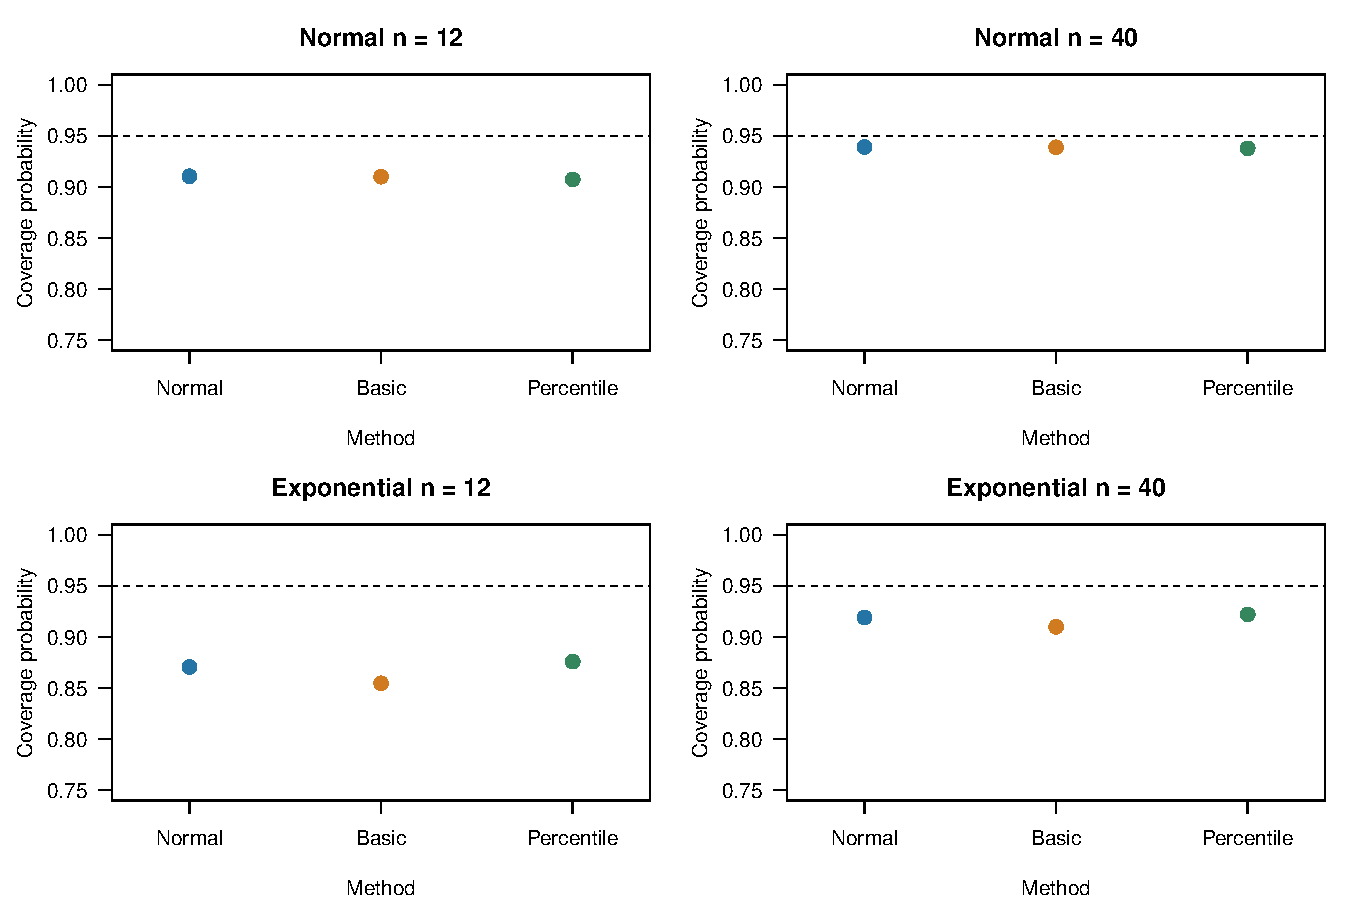
\includegraphics[width=\linewidth]{../output/figures/simulation-coverage.pdf}
    \end{column}
\end{columns}
\end{verbatim}
    \item \textbf{Trình bày code R bằng \texttt{semiverbatim} hoặc gói \texttt{listings}:} Cần thêm tùy chọn \texttt{[fragile]} vào \texttt{\textbackslash begin\{frame\}[fragile]} để Beamer không báo lỗi phân tích cú pháp khi biên dịch mã nguồn.
\end{enumerate}

\end{document}
